% !TeX spellcheck = en_GB
% ***************************************************** %
\section{Introduction}\label{sc:intro}
% ***************************************************** %

% problem identification
% solutions

This report summarizes the analysis performed in order to investigate the behaviour of the algorithms retrieved from the scientific literature. The optimization problem that we aim to solve is that of the Logistic Regression with $\ell_2\text{-regularization}$ term added.

The implemented algorithms are
\begin{itemize}
\item Mini-batch Gradient Descent with fixed and decreasing step-size, algorithm~\vref{code:SGD-fix-decr};
\item Mini-batch Gradient Descent with Armijo-type line search, algorithm~\vref{code:SGD-Armijo};
\item Mini-batch Gradient Descent with fixed step-size and momentum, algorithm~\vref{code:SGDM};
\item Mini-batch Gradient Descent with with Armijo-type line search and momentum correction and restart, algorithms~\ref{code:MSL-SGDM-C} and~\vref{code:MSL-SGDM-R}.
\end{itemize}

After that, the efficiency of the algorithms is tested on different datasets.

In this section the Machine Learning (ML) problem and the relative optimization problem are shown shown, proving the existence and uniqueness of the optimal solution.

% ---------------------------------------------------- %
\subsection{Classification task}
% ---------------------------------------------------- %

Given a dataset as follows
\[
\mathcal{D}=\set{(x^{(i)},\,y^{(i)})\mid x^{(i)}\in\mathcal{X},\,y^{(i)}\in\mathcal{Y},\,i=1,2,\dots,N}
\]
the general machine learning optimization problem in the context of \emph{supervised learning} is formulated as follows
\[
\min_{w}\func(w)=L(w)+\lambda\Omega(w)\rightarrow
\begin{cases}
L(w)=\frac{1}{N}\sum_{i=1}^N\ell_i(w) \\[0.5ex]
\Omega_{\ell_2}=\frac{1}{2}\norma{w}_2^2
\end{cases}
\]
where $L(w)$ is called \emph{loss function} and $\Omega(w)$ it's the \emph{regularization term} with its coefficient $\lambda$. There are three regularization possible choices, the $\ell_2$ regularization was chosen for the problem that we want to address. The vector $w$ contains the model weights associated to the dataset features.

The task performed is the \emph{binary classification}, where $\mathcal{Y}=\set{-1,1}$ are the allowed values for the response variable, i.e. negative and positive class; the adopted machine learning model is Logistic Regression. Every ML model has its loss function, the logistic regression uses the \emph{log-loss}, for a sample of the dataset the loss function is as follows
\begin{equation}\label{eq:sample_loss}
\ell_i(w)=\log\bigl(1+\exp(-y^{(i)}w^Tx^{(i)})\bigr)
\end{equation}
figure~\vref{subfig:log-loss} shows a plot of the loss function where $u=y^{(i)}$ and $v=w^Tx^{(i)}$, so the resulting function $\ell(uv)=\log\bigl(1+\exp(-uv)\bigr)$.

% ---------------------------------------------------- %
\subsection{Optimization problem}
% ---------------------------------------------------- %

Putting together the loss function and the regularization term, we can obtain the optimization problem that we want to solve using Stochastic Gradient Descent (SGD) algorithm variants
\begin{equation}\label{eq:opt-prob}
\min_{w\in\R^{(p+1)}}\func(w)=\frac{1}{N}\sum_{i=1}^N\log\bigl(1+\exp(-y^{(i)}w^Tx^{(i)})\bigr)+\lambda\frac{1}{2}\norma{w}^2
\end{equation}
where $i=1,\dots,N$ are the dataset samples, $\mathcal{X}\subseteq\R^{(p+1)}$ where $p+1$ means that there are $p$ features and the intercept. The $1/N$ term isn't always used, we choose to use that term for scaling issues. We define the matrix associated to the dataset and the model weights as follows
\[
X^T=
\begin{pmatrix}
1 & x_1^{(1)} & x_2^{(1)} & \dots & x_p^{(1)} \\
1 & x_1^{(2)} & x_2^{(2)} & \dots & x_p^{(2)} \\
\vdots & \vdots & \vdots & \ddots & \vdots \\
1 & x_1^{(N)} & x_2^{(N)} & \dots & x_p^{(N)}
\end{pmatrix}\in\R^{N\times(p+1)}\qquad
x^{(i)}=
\begin{pmatrix}
1 \\ x_1^{(i)} \\ x_2^{(i)} \\ \vdots \\ x_p^{(i)}
\end{pmatrix}\quad
w=
\begin{pmatrix}
b \\ w_1 \\ w_2 \\ \vdots \\ w_p
\end{pmatrix}
\]
the constant column is added for the intercept, also known as \emph{bias}, as the $b$ weight in vector $w$.% We can see that every $x^{(i)}$ is a column vector

The objective function $f\colon\R^{(p+1)}\to\R$ is of class $f\in C^2(\R^{(p+1)})$, we compute the first and second order derivatives
\begin{subequations}\label{eq:f-df-ddf}
\begin{align}
\func(w) &= \frac{1}{N}\sum_{i=1}^N\log\bigl(1+\exp(-y^{(i)}w^Tx^{(i)})\bigr)+\lambda\frac{1}{2}\norma{w}^2 \label{subeq:obj-fun} \\
\nabla\func(w) &= \frac{1}{N}X^Tr+\lambda w \label{subeq:jacobian} \\
\nabla^2\func(w) &= \frac{1}{N}XDX^T+\lambda I_{(p+1)}\label{subeq:hessian}
\end{align}
\end{subequations}
where $r\in\R^N$ is a vector of the same length as the total number of sample, whose elements are $r_i=-y^{(i)}\sigma(-y^{(i)}w^Tx^{(i)})$, note that $\sigma(z)$ is the sigmoid function as shown in figure~\vref{subfig:sigmoid}, $D\in\R^{N\times N}$ is a diagonal matrix whose elements are $d_{ii}=\sigma(y^{(i)}w^Tx^{(i)})\sigma(-y^{(i)}w^Tx^{(i)})$ which implies $d_{ii}\in(0,1)$, and $I_{(p+1)}$ is the identity matrix with size $p+1$.

%\[
%\begin{array}{@{}l@{}}
%\nabla\func(w)=\frac{1}{N}X^Tr+\lambda w,\quad r_i=-y^{(i)}\sigma(-y^{(i)}w^Tx^{(i)}),\,r\in\R^N \\[1ex]
%\nabla f_i(w)=\frac{1}{N}x^{(i)}r_i+\lambda w \\[1ex]
%\nabla^2\func(w)=\frac{1}{N}XDX^T+\lambda I_{(p+1)},\quad d_{ii}=\sigma(y^{(i)}w^Tx^{(i)})\sigma(-y^{(i)}w^Tx^{(i)}),D\in\R^{N\times N}
%\end{array}
%\]

%\[
%\nabla\func(w)=\frac{1}{N}X^Tr+\lambda w,\quad r_i=-y^{(i)}\sigma(-y^{(i)}w^Tx^{(i)})
%\]

%\[
%\nabla^2\func(w)=\frac{1}{N}XDX^T+\lambda I,\quad d_{ii}=\sigma(y^{(i)}w^Tx^{(i)})\sigma(-y^{(i)}w^Tx^{(i)})
%\]
%$r\in\R^N$, $D\in\R^{N\times N}$

The next proposition allows to address the optimization problem.

\begin{prop}
Problem~\eqref{eq:opt-prob} admits a unique optimal solution.
\end{prop}
\begin{proof}
We need to prove the existence and the uniqueness of the global minimum.

\noindent$(i)$ \emph{Existence} of a optimal solution. The problem is quadratic and the objective function is coercive, in fact $\forall\set{w^k}$ such that $\lim_{k\to\infty}\norma{w^k}=\infty$ holds
\[
\lim_{k\to\infty}\func(w^k)\geq\lim_{k\to\infty}\lambda\frac{1}{2}\norma{w^k}^2=\infty\Rightarrow\lim_{k\to\infty}\func(w^k)=\infty
\]
hence by a corollary of the Weirstrass theorem (see theorem~\vref{cor:weirs1}) the problem admits global minimum in $\R^{(p+1)}$.

\noindent$(ii)$ \emph{Unicity} of the optimal solution. We now prove that the hessian matrix~\eqref{subeq:hessian} is positive definite
\[
w^T\nabla^2\func(w)w=w^TXDX^Tw+\lambda w^TIw=\underbrace{y^TDy}_{\geq0}+\lambda\norma{w}^2\geq\lambda\norma{w}^2>0\quad\forall w
\]
the hessian matrix positive definite implies that the objective function is strictly convex (see definition~\ref{def:conv_fun}) and that implies that the global minimum, if exists, is unique (see proposition~\ref{prop:min_unique}). Being in the convex case, the global minimum is a $w^\ast\in\R^{(p+1)}$ such that $\nabla\func(w^\ast)=0$ (see proposition~\ref{prop:opt_second}).\qedhere
\end{proof}

\begin{rmk}
Since the log-loss is convex, the regularization term makes the objective function \emph{strongly convex}, this should speed up the optimization process.
\end{rmk}

%\begin{rmk}
%further more we can assume that $\nabla\func(w)$ is Lipschitz-continuous with constant $L$
%\end{rmk}

%\begin{itemize}
%\item the hessian matrix is positive defined $\forall w$, this means that the objective function, which is quadratic, is coercive and for the continuity that function admits global minimum, so $\func(w)$ has finite inferior limit
%\item the hessian matrix being positive defined implies also that the objective function is strictly convex (on the other hand the loss function is just convex, due to its hessian matrix being positive semi-defined), this implies that if the global minimum exists, that solution is unique
%\item a global minimum is a point that satisfy $\nabla\func(w^\ast)=0$, which is a sufficient condition implied by the convexity of the problem, see figure~\vref{subfig:log-loss}
%\item the $\ell_2$ regularization implies that the objective function is strongly convex, this speeds up the convergence
%\item further more we can assume that $\nabla\func(w)$ is Lipschitz-continuous with constant $L$
%\end{itemize}

%\[
%y=
%\begin{pmatrix}
%y^{(1)} \\ y^{(2)} \\ \vdots \\ y^{(N)}
%\end{pmatrix}\in\set{-1,1}
%\]

%\[
%\begin{array}{ll}
%%\func(w)\in\R & \nabla\func(w)\in\R^{(p+1)} \\
%\func(w)=\sum_{i=1}^N\log\bigl(1+\exp(-y^{(i)}w^Tx^{(i)})\bigr) & f_i(w)=\log\bigl(1+\exp(-y^{(i)}w^Tx^{(i)})\bigr) \\
%\nabla f_i(w)=\frac{1}{N}x^{(i)}r_i+\lambda w
%\end{array}
%\]

%\begin{figure}
%\centering
%\begin{tikzpicture}
%\begin{axis}[xlabel=$uv$,ylabel=$\ell$]
%\addplot[samples=200,blue,smooth] {ln(1+exp(-x))};
%\addplot[dotted] {0};
%\end{axis}
%\end{tikzpicture}
%\caption{Log-loss}
%\label{fig:log-loss}
%\end{figure}

%\begin{figure}
%\centering
%\subfloat[][\emph{Log-loss, see equation~\eqref{eq:sample_loss}. If $uv\gg0$ then the example is labelled correctly; if $uv\ll0$ then the label is the wrong one.}\label{subfig:log-loss}]%
%{\begin{tikzpicture}
%\begin{axis}[xlabel=$uv$,ylabel={$\ell(uv)$},axis lines=middle,enlargelimits,width=0.45\textwidth]
%\addplot[samples=200,blue,smooth] {ln(1+exp(-x))};
%\addplot[dashed] {1};
%\end{axis}
%\end{tikzpicture}} \quad
%\subfloat[][\emph{Sigmoid function}\label{subfig:sigmoid}]%
%{\begin{tikzpicture}
%\begin{axis}[xlabel=$z$,ylabel={$\sigma(z)$},axis lines=middle,enlargelimits,width=0.45\textwidth]
%\addplot[samples=200,red,smooth] {1/(1+exp(-x))};
%\addplot[dashed] {1};
%\end{axis}
%\end{tikzpicture}}
%\caption{Log-loss and sigmoid function plots}
%\label{fig:log-sigma}
%\end{figure}

%\begin{figure}
%\centering
%\begin{tikzpicture}
%\begin{axis}[xlabel=$uv$,ylabel={$\ell(u,v)$},axis lines=middle,enlargelimits,width=0.45\textwidth,legend style={nodes={scale=0.5, transform shape}}]
%\addplot[samples=200,blue,smooth] {ln(1+exp(-x))+0.5*x^2};
%\addplot[samples=200,red,smooth] {ln(1+exp(-x))+0.5*0.5*x^2};
%\addplot[samples=200,green,smooth] {ln(1+exp(-x))+0.5*0.1*x^2};
%\addplot[dashed] {1};
%\legend{$\lambda=1$, $\lambda=0.5$, $\lambda=0.1$}
%\end{axis}
%\end{tikzpicture}
%\caption{Influence of the regularization term on the objective function~\eqref{eq:opt-prob}}
%\label{fig:loss_regul}
%\end{figure}

\begin{figure}
\centering
\subfloat[][\emph{Log-loss, equation~\eqref{eq:sample_loss}. If $uv\gg0$ then the example is labelled correctly; if $uv\ll0$ then the label is the wrong one.}\label{subfig:log-loss}]%
{%
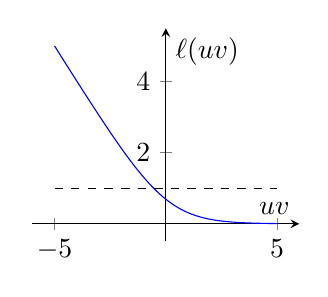
\begin{tikzpicture}
\begin{axis}[xlabel=$uv$,ylabel={$\ell(uv)$},axis lines=middle,enlargelimits,width=0.41\textwidth]
\addplot[samples=200,blue,smooth] {ln(1+exp(-x))};
\addplot[dashed] {1};
\end{axis}
\end{tikzpicture}%
} \quad
\subfloat[][\emph{Influence of the regularization term on the loss function, equation~\eqref{subeq:obj-fun}, $\lambda=\textcolor{blue}{1},\textcolor{red}{0.5},\textcolor{green}{0.1}$}\label{subfig:loss_regul}]%
{%
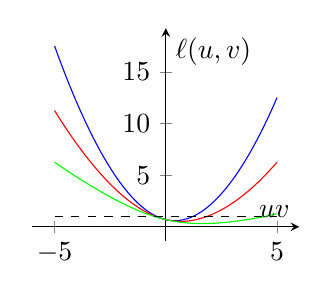
\begin{tikzpicture}
\begin{axis}[xlabel=$uv$,ylabel={$\ell(u,v)$},axis lines=middle,enlargelimits,width=0.41\textwidth,legend style={nodes={scale=0.5, transform shape}}]
\addplot[samples=200,blue,smooth] {ln(1+exp(-x))+0.5*x^2};
\addplot[samples=200,red,smooth] {ln(1+exp(-x))+0.5*0.5*x^2};
\addplot[samples=200,green,smooth] {ln(1+exp(-x))+0.5*0.1*x^2};
\addplot[dashed] {1};
%\legend{$\lambda=1$, $\lambda=0.5$, $\lambda=0.1$}
\end{axis}
\end{tikzpicture}
} \quad
\subfloat[][\emph{Sigmoid function}\label{subfig:sigmoid}]%
{%
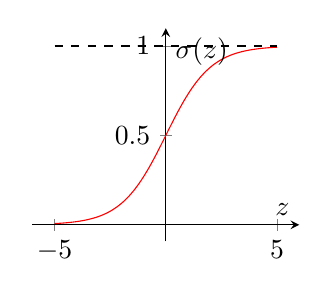
\begin{tikzpicture}
\begin{axis}[xlabel=$z$,ylabel={$\sigma(z)$},axis lines=middle,enlargelimits,width=0.41\textwidth]
\addplot[samples=200,red,smooth] {1/(1+exp(-x))};
\addplot[dashed] {1};
\end{axis}
\end{tikzpicture}%
}
\end{figure}

%\begin{itemize}
%\item $uv\gg0$: the example is labelled correctly
%\item $uv\ll0$: the class assigned to the example is the wrong one
%\end{itemize}
